
\begin{figure}
	\centering
	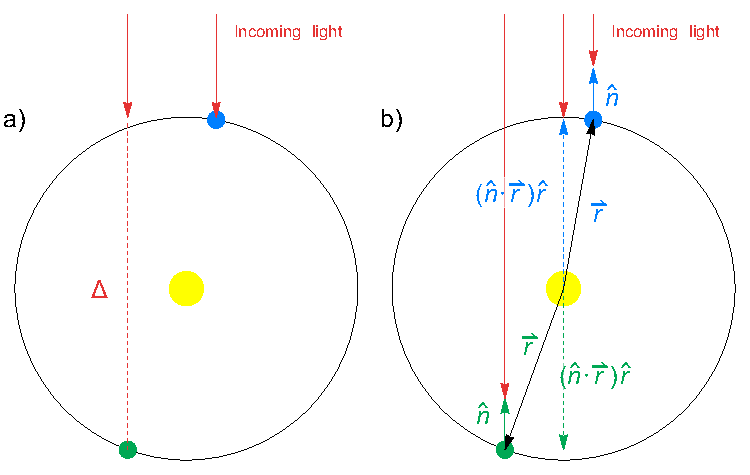
\includegraphics[width=0.9\textwidth]{img/Heliocentric.pdf}
	%\captionsetup{width=\textwidth}
	\caption[Conceptual view of the R\o{}mer delay]{ Conceptual view of the R\o{}mer delay for a signal coming from above (in red). 
	The comparison is made between the earth at two points of its orbit (blue and green disks) around the sun (yellow disk).
	\textbf{a)} The distance $\Delta$ that the incoming light has to travel if the earth is in the opposite side of its orbit (green earth) will mean a time delay of $\Delta/c$
	relative to the nearest part of the orbit (blue earth).
	The limit value for $\Delta$ is $\sim2$ AU, so the time delay would be around $16$ minutes.
	\textbf{b)} This time the excess distance is calculated from the sun, and its value is the projection of the sun-to-earth vector to the vector normal to the incoming signal.
	}
	\label{fig:romer-delay}
\end{figure}


\begin{figure}
	\centering
	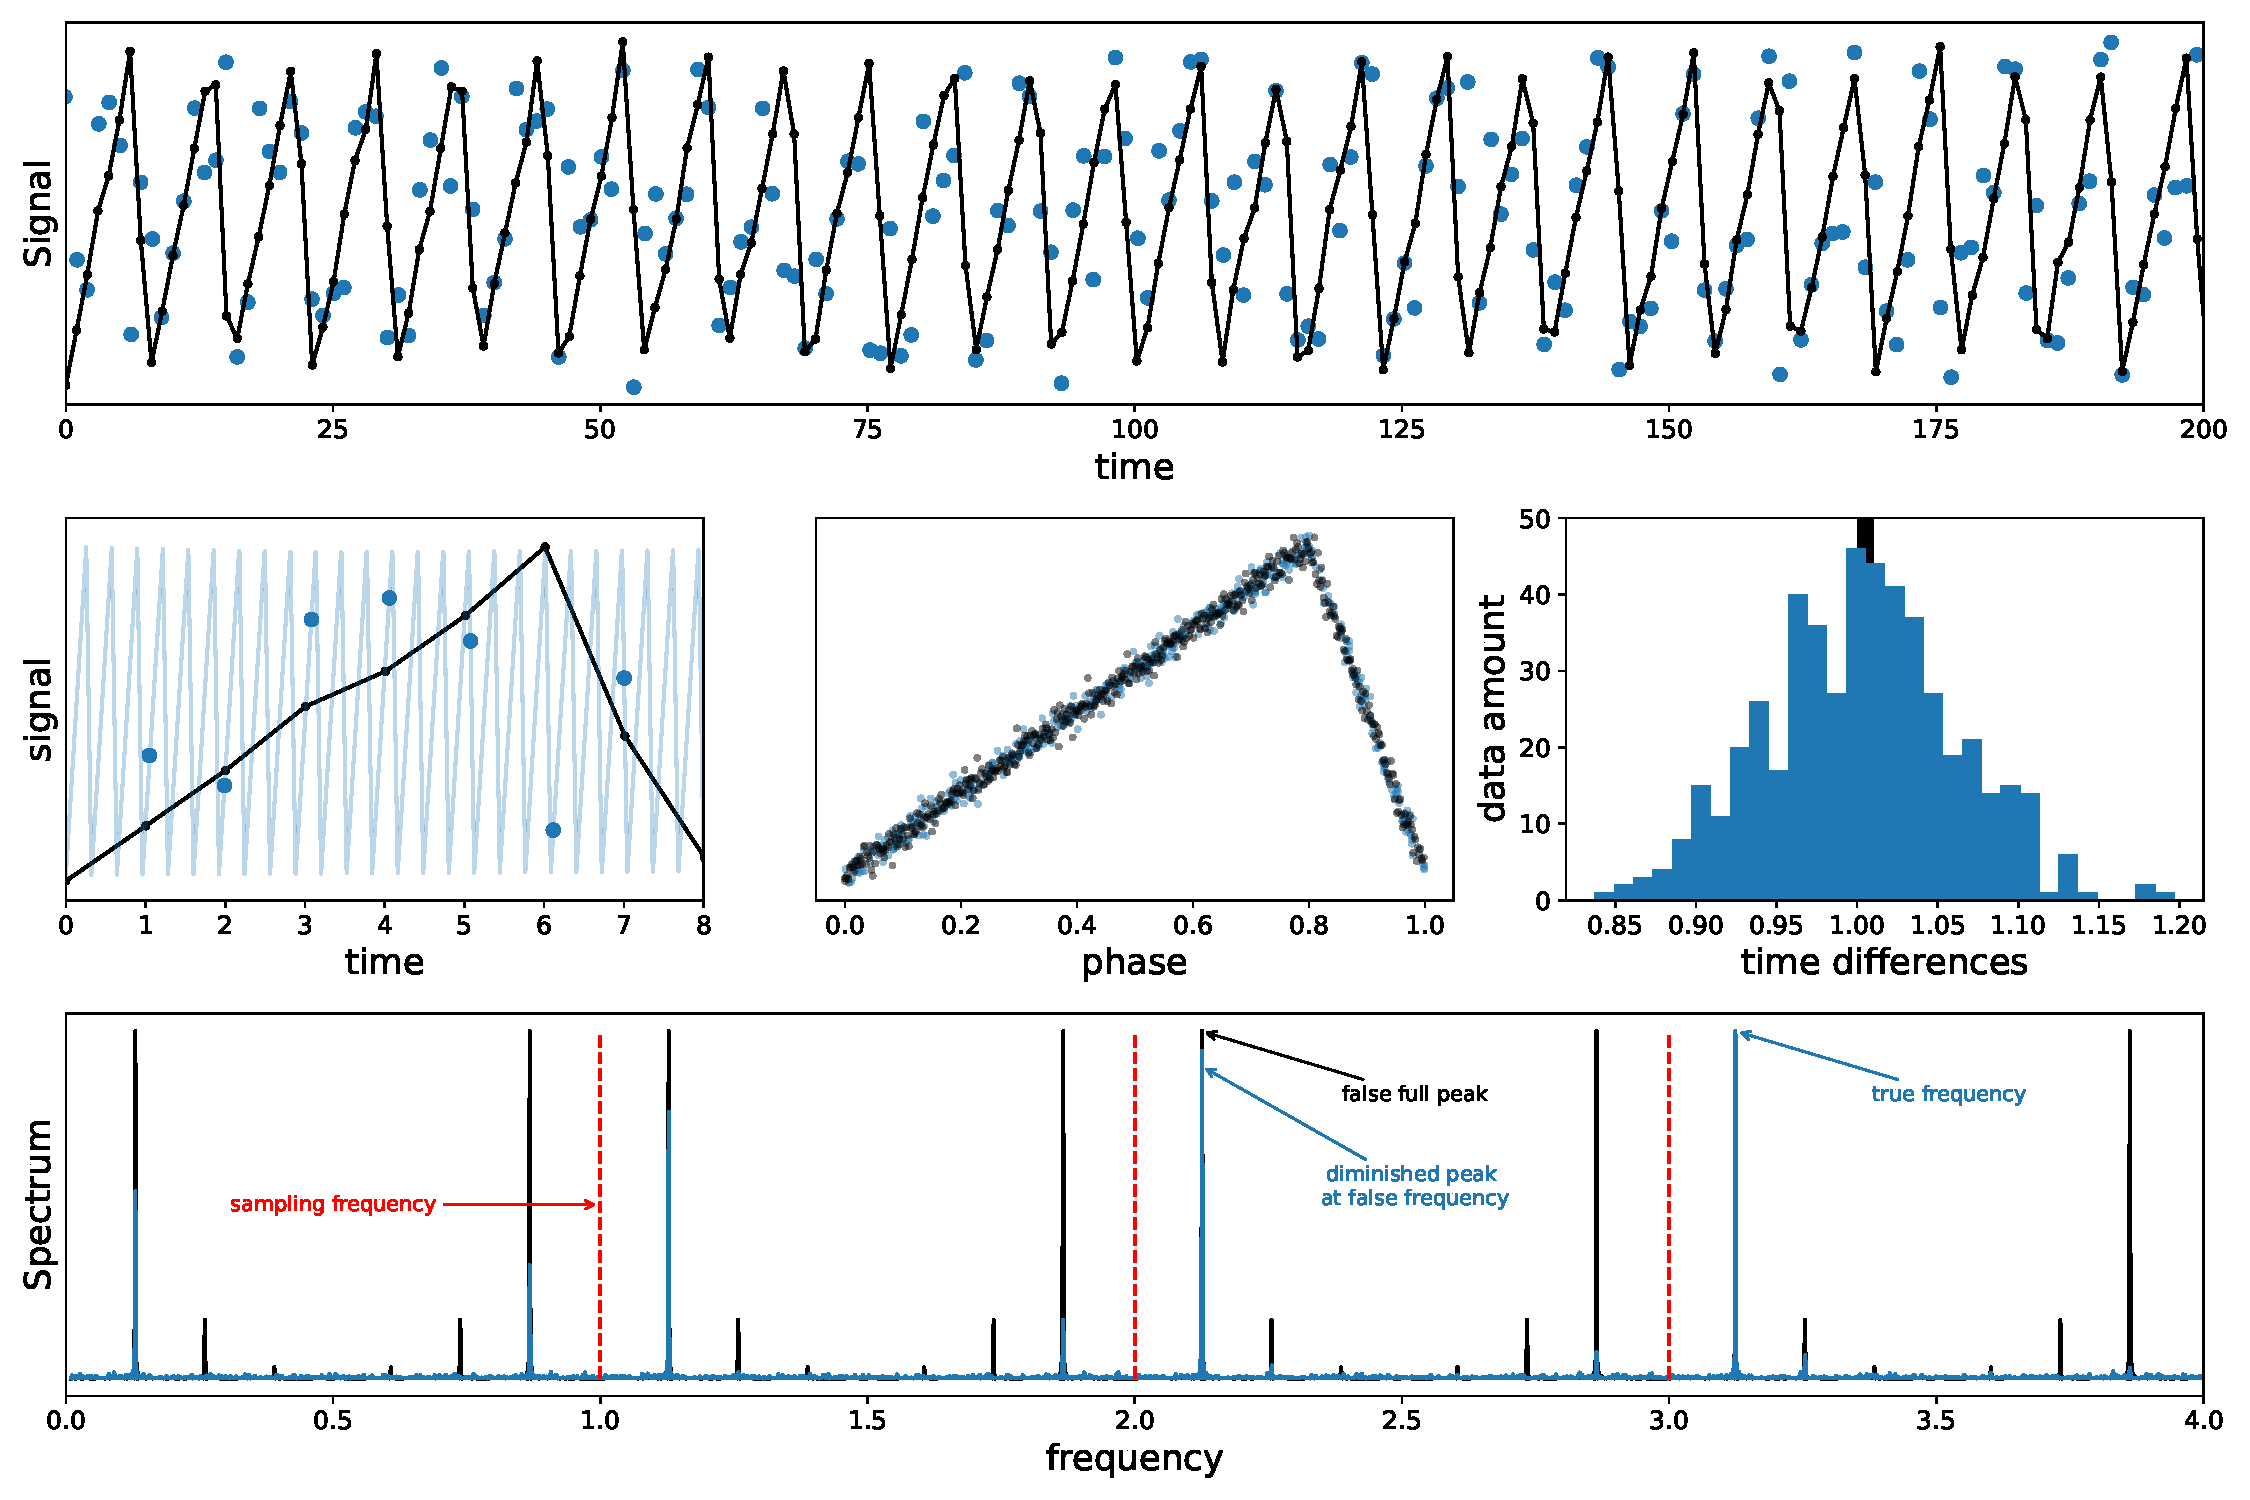
\includegraphics[width=\textwidth]{img/uneven_advantage.pdf}
	\caption[Comparison between even and uneven sampled signal past the Nyquist limit]{
		Sample skewed triangular wave sampled two ways: the black dots are sampled one each unit of time.
		The sample times of the blue dots are very near one sample each unit of time, but have a little dispersion,
		as can be seen in the left histogram.
		The frequency of the generated data is 3.124 time units.
		It is clear that the spectrum reflects every half of the sampling time (Nyquist frequency). 
		On the uneven sampling case, the spectrum does not reflect exactly; there are peaks greater than others,
		and the differences last until several times past the sampling frequency.
		The greatest peak is in the correct frequency, and the rest are partially canceled out.
		This cancellation augments with the dispersion on the sampling times, and the number of data.
		The detailed curve on the mid-left shows how exactly this happens: if the frequency is high, 
		the dots with take an entire different path on the curve with the slightest of the temporal deviations.
	}
	\label{fig:uneven-advantage}
\end{figure}


\begin{figure}
	\centering
	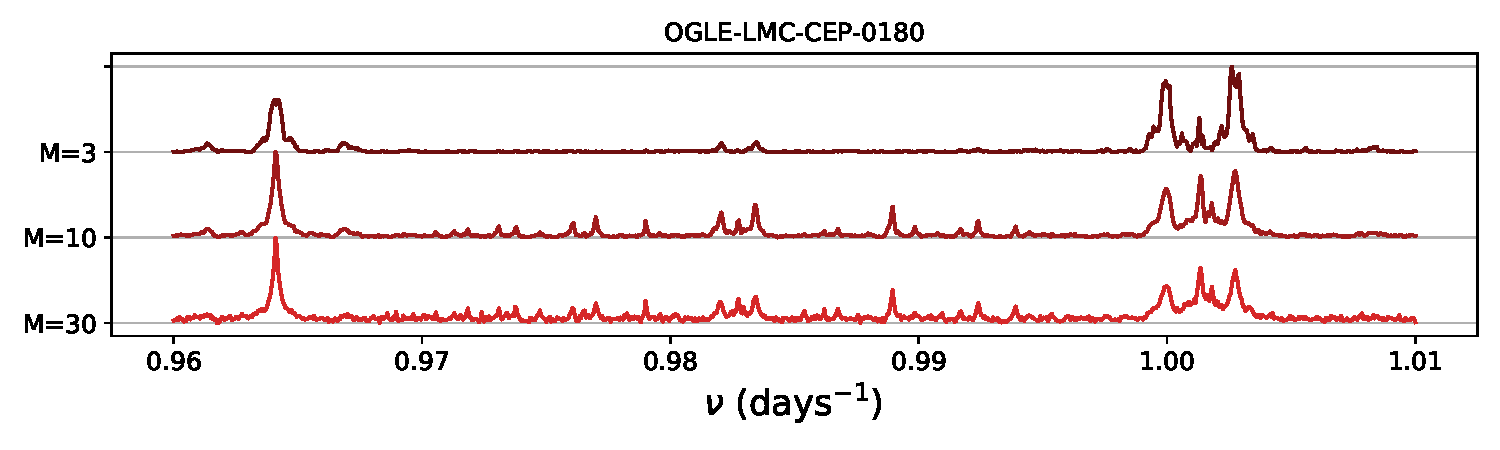
\includegraphics[width=\textwidth]{img/entropy_bins.pdf}
	\caption[Example of zone number dependency for the entropy method]{
		Entropy method applied to the same star over the same interval, but with varying number of zones per axis.
		The total number of zones would be $m=M^2$. 
		The first peak that can be observed at around $\nu=0.965$/day is the correct frequency for this star.
		The peaks near $\nu=1$/day are alias peaks, explained on \autoref{fig:problem}.
		The lower the number of zones, the higher the alias peaks compared to the true peak.
		At low number of zones there is also considerably less noise with respect to the Fourier spectrum 
		(see \autoref{fig:examples} for a comparison), and the process of taking the entropy is faster.
		This compromise between speed, noise levels and false peak heights should be taken into account 
		for any application of the entropy periodogram, unless a way to eliminate the false peaks is found,
		as in the case of the Fourier, Lomb-Scargle and dispersion periodograms.
	}
	\label{fig:entropy-alias}
\end{figure}

\begin{figure}
	\centering
	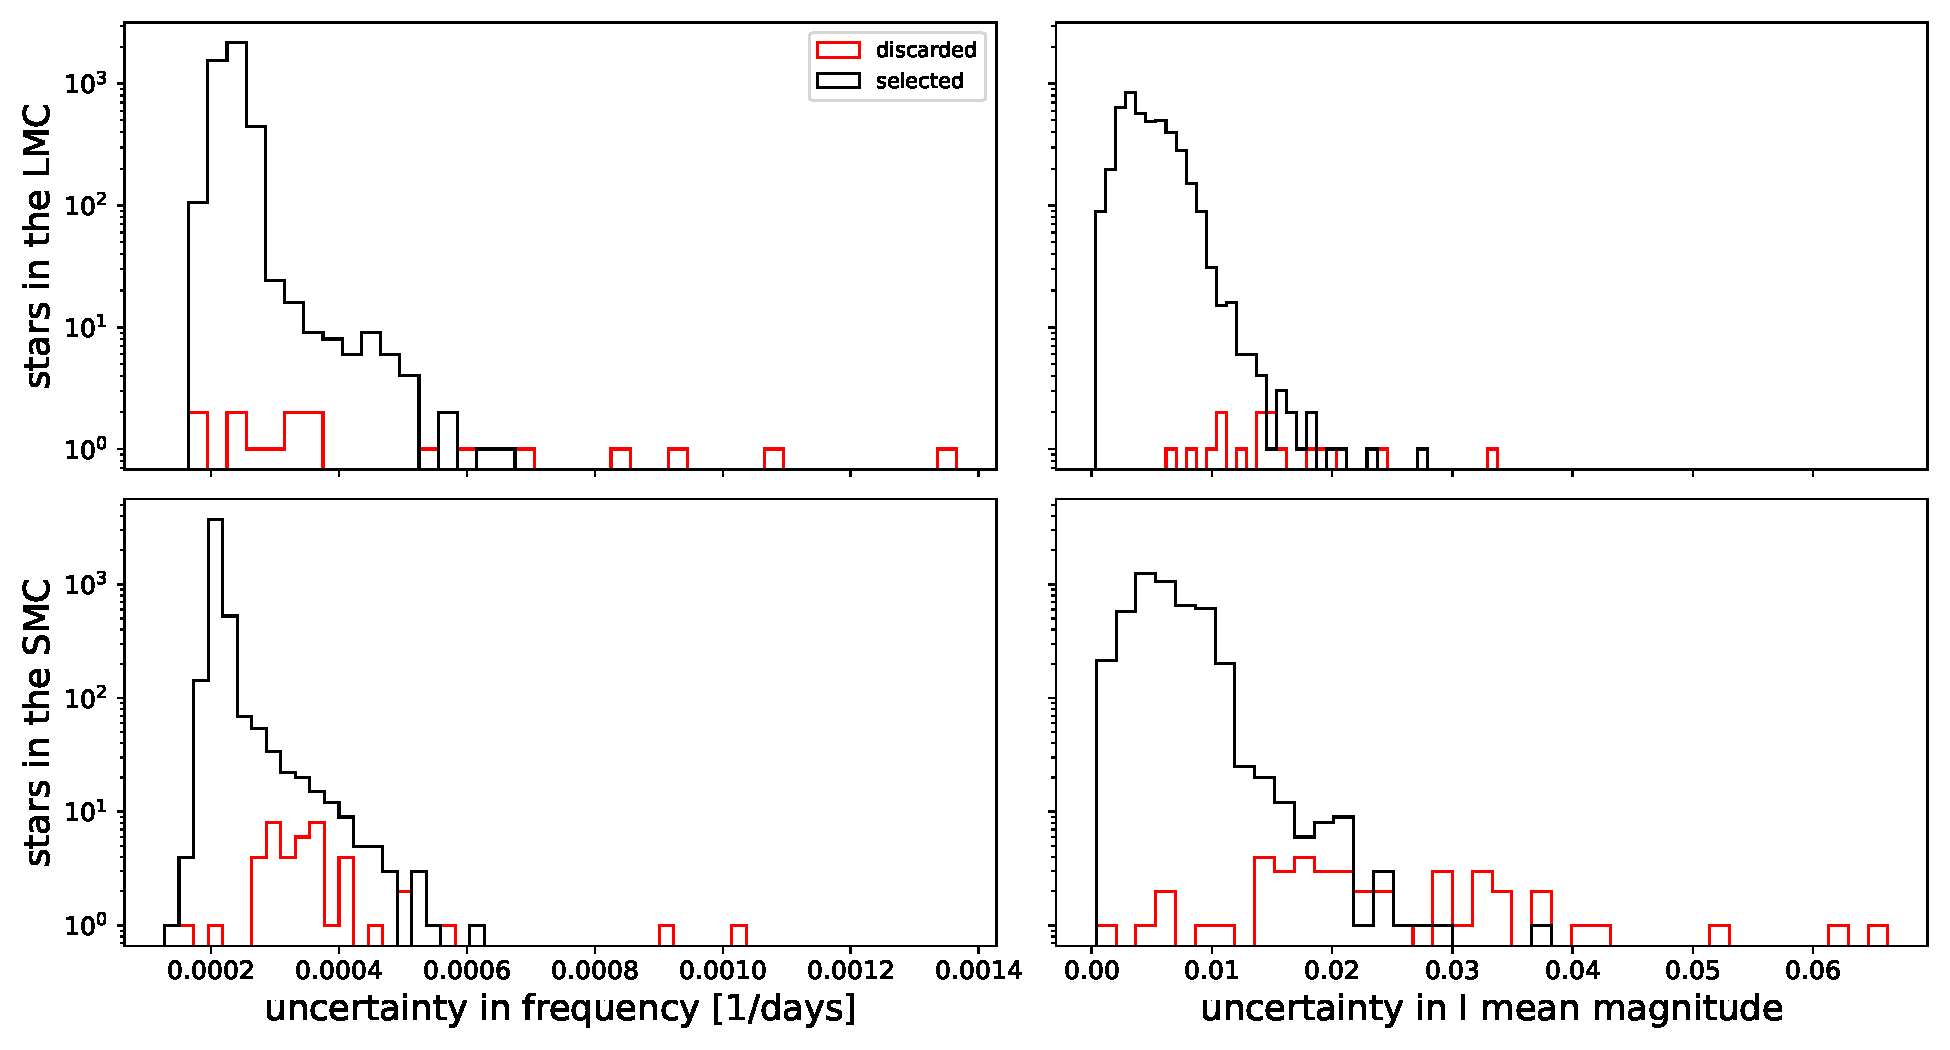
\includegraphics[width=\textwidth]{img/results_uncertainties.pdf}
	\caption[Uncertainties in the PL relation for the processed stars]{
		Distribution of uncertainties on calculations for the PL diagram, for the selected (black) and discarded (red) stars on each cloud, 
		according to the criteria discussed on \autoref{fig:peaks-n-points}.
		The uncertainty of the peaks are their full width at half maximum, 
		and the uncertainties in mean magnitude were calculated with a combination of pooled variance from each measurement and statistical bootstrap.
	}
	\label{fig:uncertainties}
\end{figure}


\begin{figure}
	\centering
	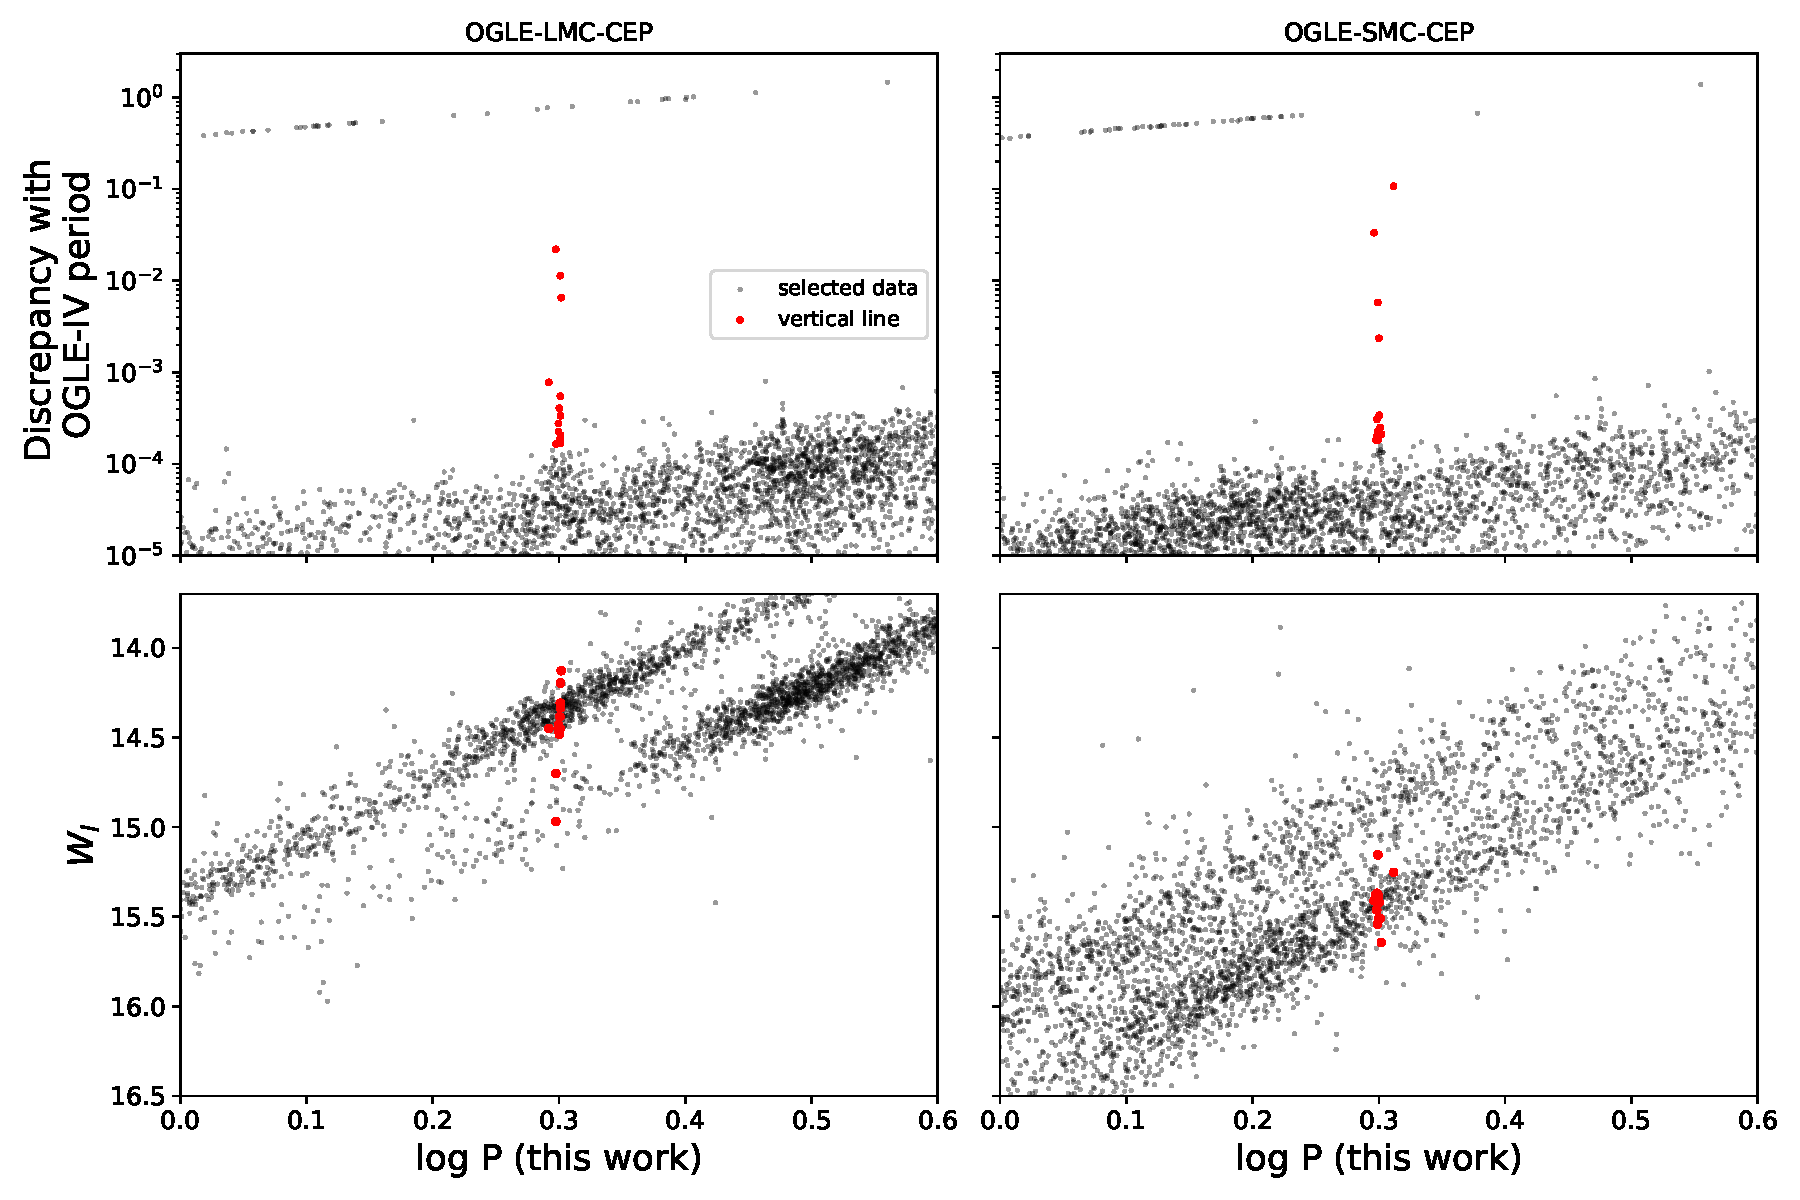
\includegraphics[width=\textwidth]{img/vertial_line_detail.pdf}
	\caption[Detail of the vertical line on the discrepancy plot]{
		Detail of the vertical bridge between the zones of low and high discrepancy of \autoref{fig:comparison}.
		The range used to capture the stars on this vertical line, shown in red, were $-3.8<\log \Delta P < -0.8$ and $0.28 < \log P < 0.32 $.
		In the SMC case, the line curves at the end, and seemingly continues alongside the horizontal line of high discrepancy.
	}
	\label{fig:vertical-discrepancy}
\end{figure}


\begin{figure}
	\centering
	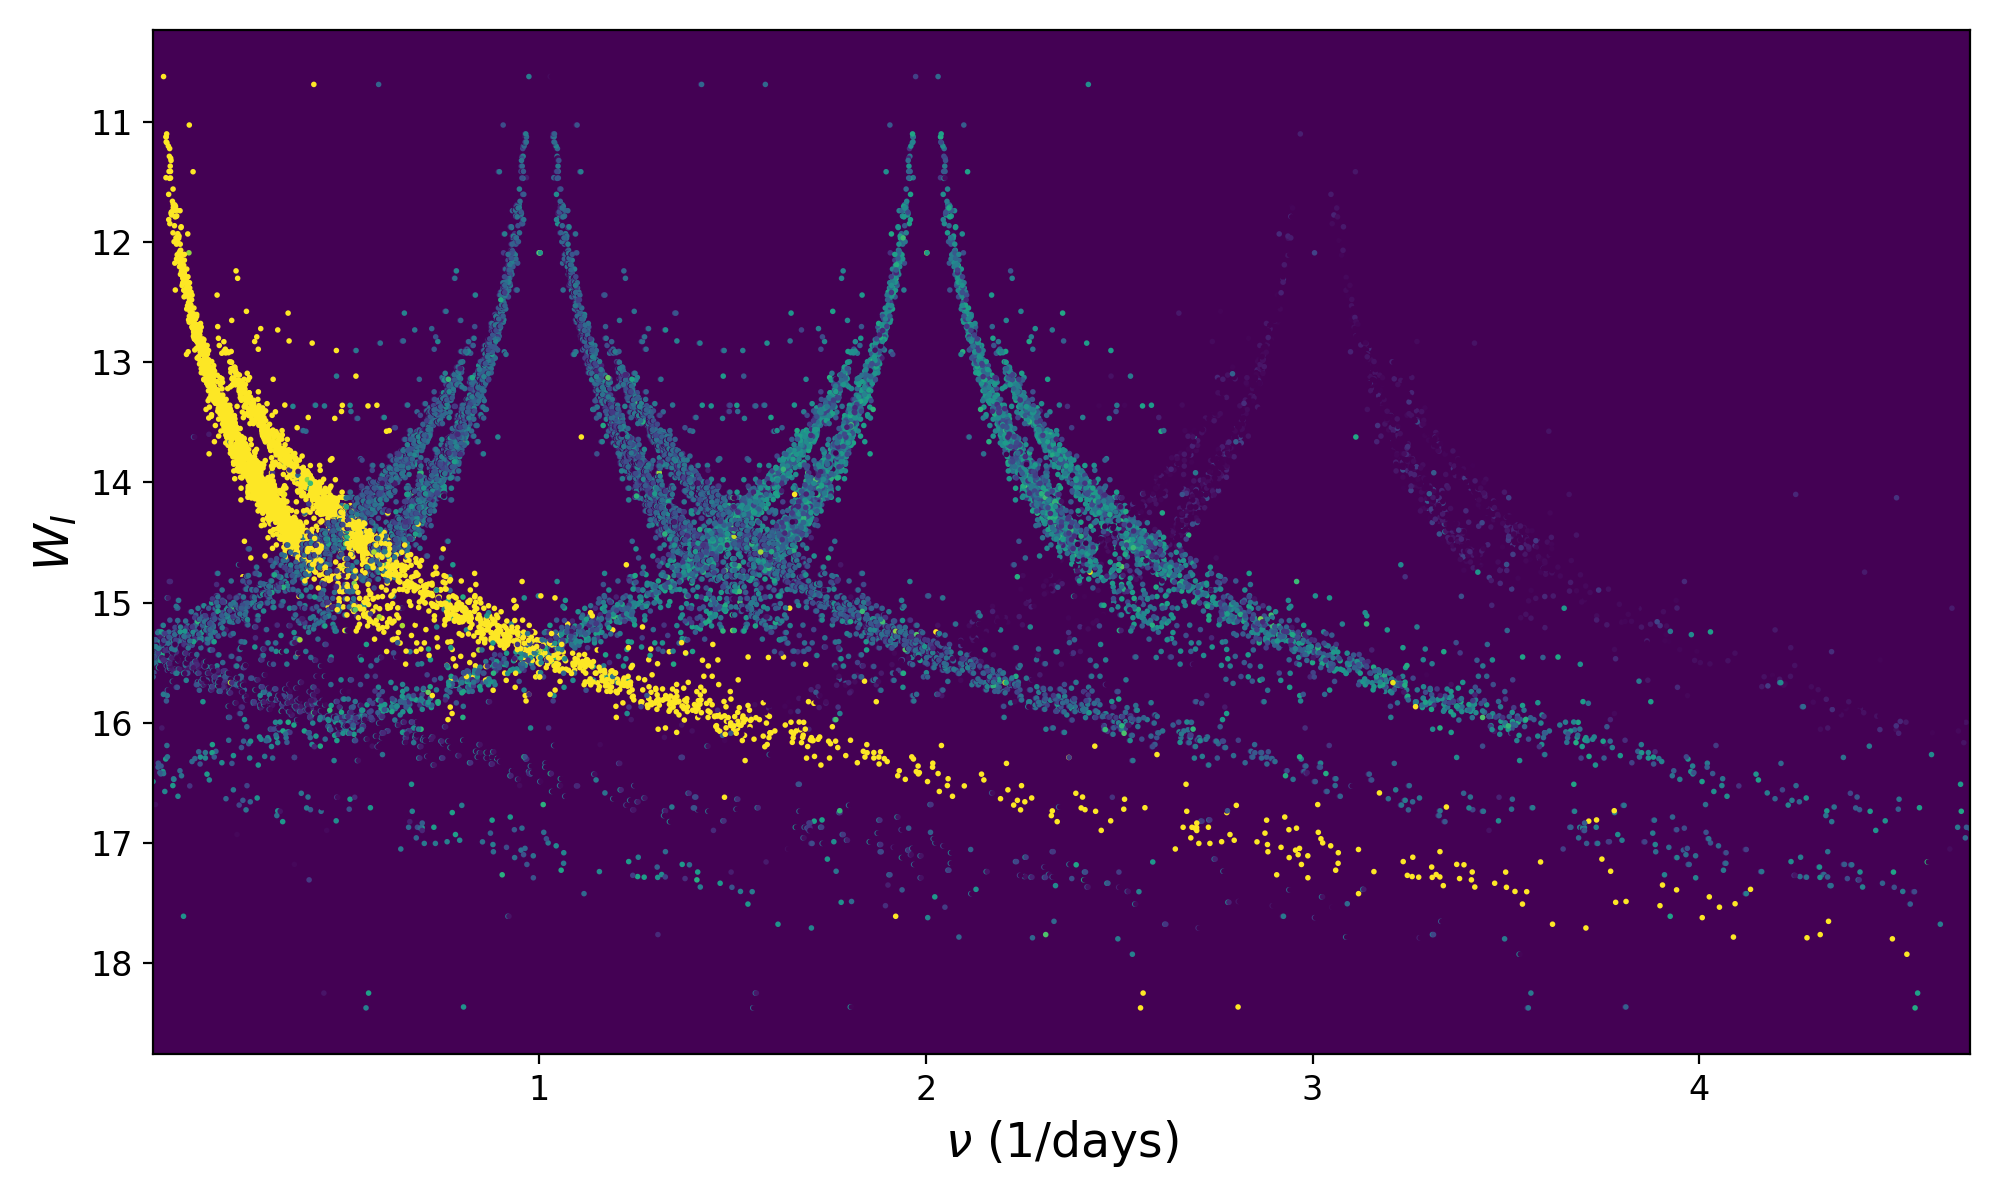
\includegraphics[width=\textwidth]{img/lmc_freq.png}
	\caption[Linear frequency PL relation with secondary peaks for the LMC]{
		PL diagram for the LMC, but the x-axis is the linear frequency grid where the periods were searched.
		Principal peaks are shown in yellow, and secondary in more bluer colors, according to their peak heights on the spectrogram.
		As the temporal cadence of the data is something around 1 day, the situation is a perfect realization of the example plots from \autoref{fig:uneven-advantage};
		the spectrograms reflect horizontally every 0.5/day, which is half the \enquote{mean} sampling frequency (modulo 1, see \autoref{fig:1234-cadence}) and 
		if it were not for the uneven sampling, all the less prominent peaks would be equal in height to the principal frequency peak.
		Effectively, for frequencies higher than 0.5 would be impossible to tell apart the true peaks from the alias ones.
	}
	\label{fig:linear-color-pl-lmc}
\end{figure}
